\section{Fine preconditioner}

Let us finally give a few explanations about the fine preconditioner and how it is implemented. Practically, in addition to the information we already have about a quadrant (the physical coordinate of its corners, the global number of the local nodes in it, if some nodes are hanging,...), we need three things to be able to compute the fine preconditioner : 

\begin{enumerate}
\item The matrices $V$, $V^{-1}$ and $\Lambda$ such that $L=V^{-1}\Lambda V$
\item For each quadrant, the global number of each neighbor
\item For each quadrant $e$, the orientation in the neighboring quadrant $d$ of the face that connects $d$ to $e$. 
\end{enumerate} 

The matrices $V$, $V^{-1}$ and $\Lambda$ are computed using the Lapack library (see \cite{lapack} for information) once we have built $L$, which is fairly simple from the theory.

The additional information needed (items 2 and 3 in the list above) is contained in $neighbors$, an array we build just for this purpose. 

In this section, we will first explain how to build $neighbors$ and then how to compute the residual in the overlaps (i.e. the parts of the subdomains that are not the quadrant) in the four different cases we can encounter. 


\subsection{Building $neighbors$}

The easiest way to know which quadrant is connected to what quadrant is to list every (oriented) edge in our mesh and sort that list so that pairs of edges are consecutive. Because we have non conforming meshes, we have to be careful though. Thanks to the fact that we only handle $1$-irregular meshes, we can say that a global edge consists of one, two or three oriented edges. One if we are on the boundary, two if the edge connects two quadrants and there are no hanging nodes on this edge, and three if we have hanging nodes on this edge. 

Thus, the first thing to do is to go through the list of quadrants and for each quadrant, build four edge structures. The structure contains the end points of the edge (oriented counter-clockwise for the quadrant), whether the edge contains hanging nodes and if so, if it is the first or the second part of the larger edge. It also contains the global number of the quadrant it is in and its disposition (0 for a west edge, 1 for an east edge, 2 for a south edge, and 3 for a north edge).

This method has still one problem that arises from hanging nodes. The best way to show is with an example. Let us assume we have the same mesh as the one in figure \ref{multi_ex_2}. When we are in quadrant 0, the north edge has end points 6 and 3. And when we are in quadrant 2, the east edge has also endpoints 3 and 6. Therefore, when we will sort the list of edges, these two will pair and we will wrongly thing that there is a connecting edge between quadrants 1 and 2. To circumvent this problem, we change the end points when we have hanging nodes. We chose negative numbers ($-1,-2,-3,-4)$ so that they do not collide with the global numbering. For example, in quadrant 1, we say that the end points of the north edge has end points $-2$ (because hanging node $b$ is on the east edge of the parent) and 3. In quadrant 2, we say that the east edge has end points 3 and $-4$ (since hanging node $a$ is on the north edge of the parent). That will allow those edges to be listed next to their right pair after sorting. However, it is important to note that we do not change the end points of the hanging edges themselves (for example the east edge in quadrant 1 and the north edge in quadrant 2). Indeed, we want them to pair with the edge that form the other part of the larger edge and for that we need them to have the same end points. 

Once we have built the list of edges, we can sort them. We will sort them first by the end points with the lowest value, then by the endpoints with the highest value and finally by their hanging information (0 if the edge is not hanging, 1 if the edge is the first part of the larger edge and 2 if it is the second). Once sorted, we can go through the list to form $neighbors$. We know that if three consecutive edges have the same end points, then the first is the larger (non hanging) edge, the second is the first part of the hanging edge and the third is the second part. If two consecutive edges have the same end points, then they connect two quadrants through a non hanging edge. If we have a lone edge, then it is part of the boundary. 

Let us define $neighbors_{i;k}$ for $i=west,east,north,south$ to be the part of $neighbors$ related to quadrant $k$ and edge $i$. Then, it is given by (with $j \in \{west,east,north,south\}$): 

\begin{align*}
neighbors_{i;k} &= \begin{bmatrix}
-1 & -1 & -1
\end{bmatrix} &\text{if edge $i$ in quadrant $k$ lies on the boundary}\\
&= \begin{bmatrix}
a & -1 & j
\end{bmatrix} &\text{if non hanging edge $i$ in quadrant $k$ connects $k$ to $a$}\\
& &\text{$a$ is connected to $k$ by non hanging edge $j$}\\
&= \begin{bmatrix}
a & b & j
\end{bmatrix} &\text{if non hanging edge $i$ in quadrant $k$ connects $k$ to $a$ and $b$}\\
& &\text{$a$ and $b$ are connected to $k$ by hanging edge $j$}\\
&= \begin{bmatrix}
a & a & j
\end{bmatrix} &\text{if hanging edge $i$ in quadrant $k$ connects $k$ to $a$}\\
& &\text{$a$ is connected to $k$ by non hanging edge $j$}
\end{align*}

We can see that any neighbor can be of four types : the boundary, a regular neighbor through a non hanging edge, two neighbors through a non hanging edge, a neighbor through a hanging edge. All those types have to be treated separately when we compute the local residual. 

Let us finally give two examples. In figure \ref{multi_ex_2}, $neighbors$ associated with the east edge in quadrant 1 is : 

$$neighbors_{east;1} = \begin{bmatrix}
4 & 4 & west
\end{bmatrix}$$

The one associated with the south edge in quadrant 5 is : 

$$neighbors_{south;5} = \begin{bmatrix}
2 & 3 & north
\end{bmatrix}$$

\subsection{Computing the local residual}
Let us now look at how to compute the local residual on a given subdomain. The part that is constituted by the quadrant is easy enough : we just look at the nodes in the quadrant and use, if necessary, the $R_{ij}^e$ operator (see the first section of this chapter for more information). It is trickier for the overlaps (i.e. the parts in the subdomain that is not a full quadrant but the layer of GLL nodes in the neighbors). As explained above, there are four different types of neighbors and all of them have to be treated individually. 

Figure \ref{fine_ex} shows the latter three kinds of neighbors a quadrant can have. We will use this example to illustrate the different cases. 

\begin{figure}
\centering
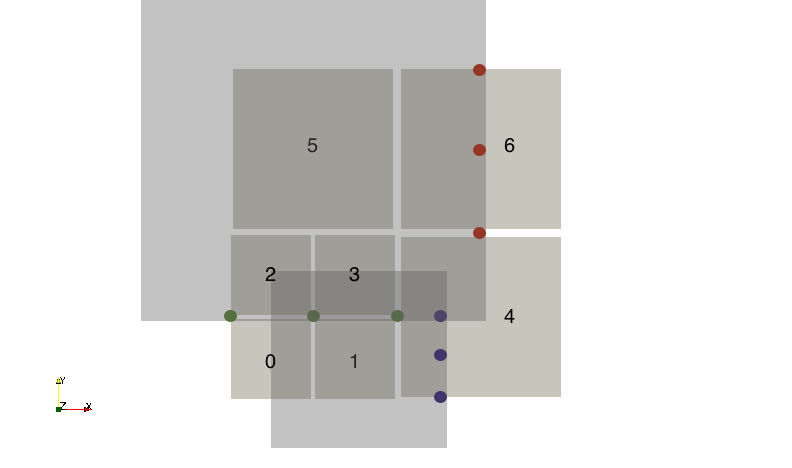
\includegraphics[scale=0.5]{Implementation/fine_ex.png}
\caption{Example of a mesh for $p=2$ and the subdomains (in light grey) associated with quadrants 1 and 5. It presents the latter three kinds of neighbors quadrants can have : one neighbor through a non hanging edge (in red for quadrant 5), two neighbors through a non hanging edge (in green for quadrant 5) and one neighbor through a hanging edge (in blue for quadrant 1).}
\label{fine_ex}
\end{figure}

\subsubsection{The neighbor is the boundary}

We know that edge $i$ of quadrant $k$ lies on the boundary if the first entry of $neighbors_{i;k}$ is $-1$. This is the easiest case to treat. As said in the theory chapter, we just fill the overlap using a linear interpolation from inside the quadrant. When we gather the fine scale correction, we of course do not take this overlap into account. 

\subsubsection{One neighbor through a non hanging edge}

That is another fairly easy case. Because of our assumptions, we can copy the values of the residual of the neighboring quadrant in the overlap. Indeed, in that case, the nodes in the overlap coincide with the local nodes of the neighboring quadrant. An example of such a case is given for quadrant 5 in figure \ref{fine_ex} (nodes in red). We can see that quadrant 6 is its neighbor through its (non hanging) east edge. We can also see that the red nodes in the overlap coincide with local GLL nodes of quadrant 6. 

There is however one problem with this approach. It does not take into account the fact that edges in quadrant 6 can be hanging. Indeed, in general, the edge between quadrants 6 and 4 could be a hanging edge. Then, it is not possible to just copy the values. Since it grows the complexity a lot, our application does not handle this case. We will see in the results chapter that the fine preconditioner works anyway. 

\subsubsection{Two neighbors through a non hanging edge}

Here, even with our assumptions, we have to interpolate the value of the residual since nodes do not coincide. An example of this situation is given in figure \ref{fine_ex} for quadrant 5 (nodes in green). For this special case of $p=2$, we can see that the nodes in the overlap do coincide with nodes in quadrant 2 and 3 but for higher degrees it is not true anymore. We therefore have to interpolate the value of the residual at the right place. It is here a two dimensional interpolation (where the interpolation for hanging nodes is one dimensional). We can note that it is always the same interpolation and we can therefore build a matrix beforehand, called $two\_to\_one$, and apply it every time we encounter this case. 

The same remark as before applies here : we do not treat every case perfectly. For example, we do not take into account the fact that the edge between quadrant 3 and 4 is hanging for the two dimensional interpolation. This yields a small error when we compute the residual for such an overlap. 

When we have to perform the gather operation, we use the transpose of $two\_to\_one$ to distribute the fine scale correction to nodes in quadrants 2 and 3. 

\subsubsection{One neighbor through a hanging edge}

This last case also needs us to interpolate the value of the residual because, here again, nodes do not coincide with local nodes in the neighboring quadrant. An example of this case is given in figure \ref{fine_ex} for quadrant 1 (nodes in blue). It is here clear that the nodes in the overlap do not coincide with local nodes in quadrant 4. Once again, we have to perform a two dimensional interpolation to get the values of the residual. It is always the same interpolation and we build the matrix $one\_to\_two$ to perform it. The transpose of this matrix is used when we have to gather the fine scale correction.

 As before, we do not handle the extra cases : for this example, that the edge between quadrant 4 and 6 could be hanging. We will see in the next chapter the consequences of this approximation on the number of iterations of PCG.

